\documentclass[12pt,a4paper]{article}
\usepackage[utf8]{inputenc}
\usepackage[T1]{fontenc}
\usepackage[spanish,mexico]{babel}
\usepackage[margin=2.5cm]{geometry}
\usepackage{graphicx}
\usepackage{float}
\usepackage{caption}
\usepackage{subcaption}
\usepackage{fancyhdr}
\usepackage{hyperref}
\usepackage{listings}
\usepackage{xcolor}
\usepackage{booktabs}
\usepackage{enumitem}

\pagestyle{fancy}
\fancyhf{}
\fancyhead[L]{Proyecto de Chat TCP}
\fancyhead[R]{Facultad de Ciencias, UNAM}
\fancyfoot[C]{\thepage}

\hypersetup{
    colorlinks=true,
    linkcolor=black,
    urlcolor=blue,
    citecolor=black
}

\title{Proyecto 1: Chat TCP}
\author{Espinosa Meléndez Juan Ernesto}
\date{\today}

\begin{document}
\thispagestyle{empty}
\begin{figure}[H]
    \centering
    \includegraphics[width=4cm]{unam-logo-png_seeklogo-144764.png}
    \hspace{2cm}
    \includegraphics[width=4cm]{FC1.png}
\end{figure}

\vspace{1cm}

\begin{center}

    {\Large \textbf{UNIVERSIDAD NACIONAL AUTÓNOMA DE MÉXICO}}\\[0.5cm]

    {\Large \textbf{FACULTAD DE CIENCIAS}}\\[1.5cm]

    {\LARGE \textbf{Proyecto 1}}\\[0.5cm]

    {\Large \textbf{Chat TCP}}\\[1.5cm]

    \textbf{Alumno:}\\
    Espinosa Meléndez Juan Ernesto\\
    No. de cuenta: 323150066\\[1cm]

    \textbf{Asignatura:}\\
    Modelado y Programación\\[0.8cm]

    \textbf{Profesor:}\\
    Canék Peláez Valdés\\[1cm]
    \textbf{Ayudantes:}\\
    Cynthia Lizbeth Sánchez Urbano\\
    Miriam Torres Bucio

\end{center}

\newpage

\tableofcontents

\newpage

\section{Introducción}
Este proyecto trata sobre el análisis, modelado y desarrollo de un chat TCP, en donde debíamos investigar como programar un servidor y 
un cliente que se pudieran comunicar entre si. Además, debíamos determinar en que lenguaje se iba a programar, en este caso se realizó 
el servidor en C y el cliente en C++, tomando en cuenta que debíamos enviar y recibir de manera interna mensajes JSON que el usuario no 
iba a poder ver ni escribir, pero en cambio el servidor si debía lidiar con ellos.\\

Una vez terminadas las bases teníamos un protocolo que se debía cumplir para crear salas privadas y una sala pública, enviar invitaciones 
y aceptarlas, solicitar la lista de usuarios en las respectivas salas, cambiar el estatus e identificarse. Durante las clases se fueron 
dando otras indicaciones que complementaron el protocolo, tales fueron los casos de definir un límite al tamaño de mensajes, ya que solo 
existía un límite en el username que podía utilizar un usuario y un límite en el nombre de las salas privadas.
\\
Este proyecto da por hecho que el programa va a funcionar adecuadamente, ya que se cuentan con las bases necesarias, siendo que lo más 
importante es el análisis, modelado y desarrollo del mismo, sin embargo como se verá más adelante, hubo distintos problemas a la hora del 
desarrollo y en la cuestión del modelado.

\section{Análisis y modelado}
\subsection{Análisis}
La elección del lenguaje fue algo que no pensé demasiado, ya que, Canek ofreció 1 punto extra si hacíamos el servidor en C y el usuario 
en un lenguaje distinto, así que opté por utilizar C en el servidor y C++ para el usuario, no solo por el punto extra que ofreció Canek, 
sino que también contaba con libros para aprender a programar en C y C++, implementar algoritmos en C y de programación estructurada en C; 
con esto como base pensé que sería sencillo utilizar estos 2 lenguajes dado que contaba con bibliografía a la mano que me podía ser de 
utilidad y además podía aspirar a 2 puntos extra.
\\\\
Antes de comenzar, busqué distintos tutoriales para saber como se hacía un servidor, adicionalmente leí como funcionaban los sockets 
porque esto era muy importante para el proyecto y era algo de lo que no tenía ni idea de como implementarlo. Afortunadamente encontré un par de tutoriales que me fueron de gran utilidad al comienzo.\\
\\
Mi idea al comienzo era realizar una interfaz y que el programa sería parecido al messenger viejito que tenía zumbidos, visualmente 
me podía dar una idea, sin embargo en la cuestión del servidor lo único que tenía claro era lo que había podido observar en los tutoriales,
 adicionalmente lo único que sabía de C y C++ era lo que había podido leer en la primera semana.
\\\\
Lo que pensé para el orden de como desarrollar el proyecto fue: comenzar el servidor hasta que aceptara conexiones y utilizar un usuario
de prueba que me permitiera asegurarme que el servidor funcionaba. En este punto pude haber hecho tests para no hacerlo manualmente pero 
la verdad no tenía idea de como hacerlas y cada vez me quedaba menos tiempo para la fecha de entrega y no tenía nada en mi repositorio más que el archivo de prueba. Posteriormente traté te hacer que el servidor fuera estable, guardara los clientes en un diccionario, funcionará la lista de usuarios conectados y pudieras cambiar tu estatus, para que una vez terminara con esto fuera de lleno con todo lo que abarcaba el protocolo respecto a salas y enviar mensajes.\\\\
El cliente en algún punto tenía que crearlo, pero lo pospuse lo más que pude ya que no había investigado tantas cosas de C++ como lo hice 
con C, cuando el cliente de prueba me dejo de ser útil lo deseche y comencé con el desarrollo de uno propio que pudiera cumplir con todo 
lo que el protocolo requería.
\\\\
Una vez que ya había comenzado, los tutoriales comenzaron a ser escasos y me guié por repositorios que habían hecho un proyecto similar o 
igual al que me pedían, sin embargo, algunos no me eran completamente de utilidad, ya que algunos limitaban la cantidad de usuarios, no 
usaban JSON o estaban hechos para windows. Por tanto los use más como una guía de lo siguiente que debía hacer, lo bueno es que en el caso del cliente al haber escogido C++ contaba con referencias mucho más útiles que para guiarme en el desarrollo del servidor en C.
\subsection{Modelado}
Traté de programar siguiendo algún patrón de diseño, claro que el que tuve más claro fue el del cliente con MVC, sin embargo para el caso 
del servidor la cosa se me complicó bastante, ya que al comienzo simplemente seguí los tutoriales y creí que me sería más fácil identificar
 cual utilizar en cada caso. Sin embargo, terminé optando por hacer todo el programa de golpe y separarlo adecuadamente cuando estuviera 
 terminado. \\\\
Entiendo que es una mala práctica y si bien llegué a separar unas cosas que me parecieron más sencillas de identificar porque no me 
convenía dejarlas juntas, en su momento creí que el loop infinito dentro del servidor sería pequeño y que solo agregaría lo indispensable. 
En la práctica terminé añadiendo todo porque cuando me dí cuenta que lo tuve que haber separado desde un inicio ya era un poco tardé y 
prioricé terminar todo antes de tratar de seguir un patrón que me facilitara las cosas.\\
\\
El tener gran parte del servidor concentrada en pocos archivos y funciones hizo que eventualmente me perdiera con facilidad y se 
complicara modificar las cosas cuando algo se rompía o no funcionaba como lo había pensado, practicamente utilizaba el ctrl + f en 
todo momento. Lo único bueno es que desde el comienzo fui dejando comentarios que me permitían saber que hacía cada parte, además de 
que los nombres de las variables los hice lo más explícitos que podía pero tratando de que fueran cortos porque me terminaría hartando 
de escribir un nombre largo y poco eficaz.
\\\\
Eventualmente realicé distintas refactorizaciones para ayudarme a encontrar con mayor facilidad las cosas, además de corregir partes
 que durante las clases alguien que había hecho algo similar recibía la indicación por parte de Canek de que estaba mal hecho, así 
 que aprovechaba para cambiarlo yo también antes de que fuera demasiado tarde.\\
\section{Descripción general del sistema}

\subsection{Arquitectura cliente/servidor}

\begin{figure}[H]
    \centering
    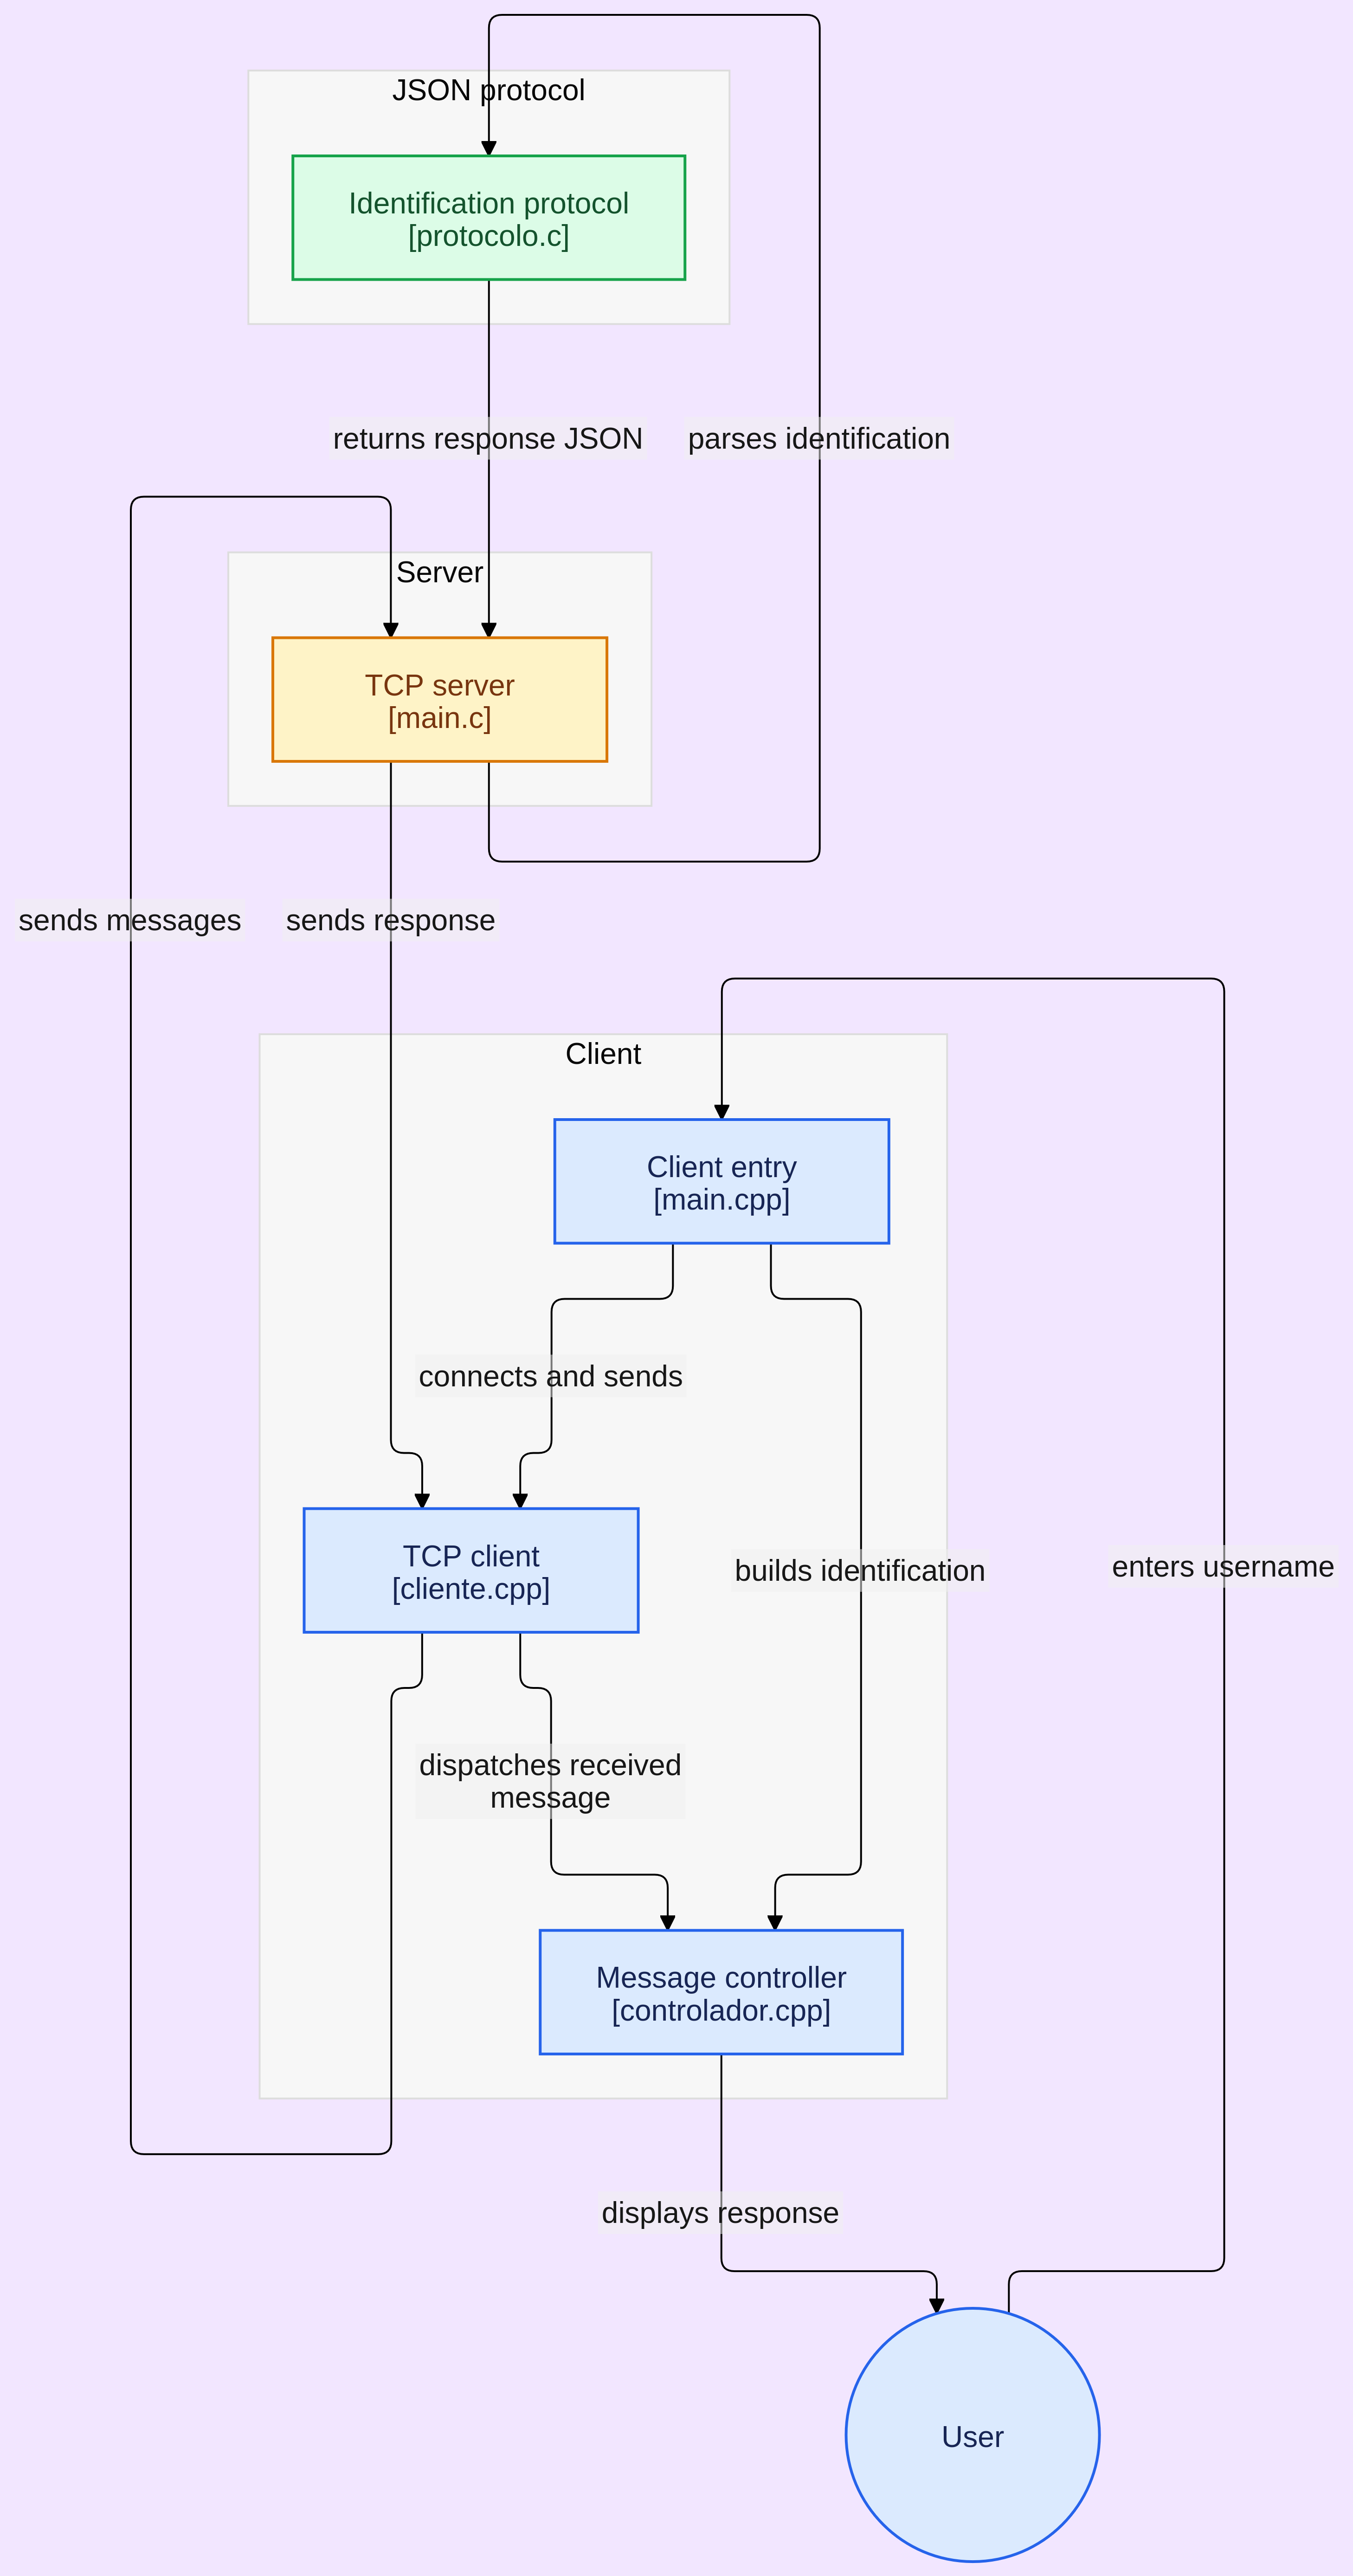
\includegraphics[width=0.55\textwidth]{diagram.png}
    \label{fig:arquitectura}
\end{figure}

\section{Protocolo de comunicación}
\subsection{Operaciones del protocolo}
\begin{table}[H]
    \centering
    \begin{tabular}{@{}ll@{}}
        \toprule
        \textbf{Operación} & \textbf{Descripción} \\
        \midrule
        IDENTIFY & Identifica al usuario ante el servidor con un nombre. \\
        STATUS & Cambia el estado del usuario (\texttt{ACTIVE}, \texttt{AWAY} o \texttt{BUSY}). \\
        USERS & Solicita la lista de usuarios conectados y su estado. \\
        TEXT & Envía un mensaje privado a otro usuario. \\
        PUBLIC\_TEXT & Envía un mensaje a todos los usuarios conectados. \\
        NEW\_ROOM & Crea una nueva sala, de la que el creador es el primer miembro. \\
        INVITE & Invita a uno o más usuarios a una sala en la que ya se es miembro. \\
        JOIN\_ROOM & Une al usuario a una sala a la que fue invitado. \\
        ROOM\_USERS & Solicita la lista de usuarios de una sala a la que se pertenece. \\
        ROOM\_TEXT & Envía un mensaje a todos los miembros de una sala. \\
        LEAVE\_ROOM & Abandona una sala de la que se es miembro. \\
        DISCONNECT & Se desconecta del chat y abandona todas sus salas. \\
        \bottomrule
    \end{tabular}
    \label{tab:operaciones}
\end{table}
\begin{table}[H]
    \centering
    \begin{tabular}{@{}ll@{}}
        \toprule
        \textbf{Mensaje} & \textbf{Descripción} \\
        \midrule
        NEW\_USER & Un nuevo usuario se identificó en el chat. \\
        NEW\_STATUS & Un usuario cambió su estado. \\
        USER\_LIST & Respuesta a \texttt{USERS}. \\
        TEXT\_FROM & Mensaje privado recibido de otro usuario. \\
        PUBLIC\_TEXT\_FROM & Mensaje público recibido de otro usuario. \\
        INVITATION & Invitación recibida a una sala. \\
        JOINED\_ROOM & Un usuario se unió a una sala. \\
        ROOM\_USER\_LIST & Respuesta a \texttt{ROOM\_USERS}. \\
        ROOM\_TEXT\_FROM & Mensaje recibido dentro de una sala. \\
        LEFT\_ROOM & Un usuario abandonó una sala. \\
        DISCONNECTED & Un usuario se desconectó del chat. \\
        RESPONSE & Resultado de una operación solicitada. \\
        \bottomrule
    \end{tabular}
    \label{tab:notificaciones}
\end{table}

\section{Implementación}

\subsection{Tecnologías utilizadas}

El servidor fue desarrollado en C y el cliente en C++. Para la comunicación
se utilizaron sockets TCP, mientras que los mensajes intercambiados entre
ambos programas se representan mediante JSON utilizando la biblioteca
json-c. El servidor utiliza además GLib para el manejo de las
tablas hash (diccionarios) empleadas en la administración de usuarios y salas.\\
Para la construcción del proyecto se utilizó Meson junto con Ninja. El
cliente utiliza las herramientas de concurrencia de C++, principalmente
std::thread, std::mutex y
\texttt{std::condition\_variable}, para recibir mensajes del servidor de
forma independiente a la interacción con el usuario.

\subsection{Requerimientos}

Para compilar y ejecutar el proyecto se requiere un sistema compatible con
sockets POSIX y contar con las siguientes herramientas y bibliotecas:

\begin{itemize}
    \item GCC y G++.
    \item Meson y Ninja.
    \item Biblioteca \texttt{json-c}.
    \item Biblioteca GLib.
\end{itemize}

El proyecto está configurado para ejecutarse localmente, utilizando
\texttt{127.0.0.1} como dirección del servidor y el puerto \texttt{1234}
para la comunicación TCP.

\subsection{Compilación y ejecución}

Desde el directorio raíz del proyecto se puede realizar la configuración
inicial y compilación mediante:

\begin{verbatim}
meson setup build
meson compile -C build
\end{verbatim}

Una vez compilado, primero se debe iniciar el servidor:

\begin{verbatim}
./build/servidor/servidor
\end{verbatim}

Posteriormente, desde otra terminal se ejecuta el cliente:

\begin{verbatim}
./build/cliente/cliente
\end{verbatim}

El cliente solicitará el nombre de usuario y, después de establecer la
conexión, permitirá utilizar las operaciones definidas en el protocolo.
Los mensajes intercambiados entre cliente y servidor se procesan
internamente como JSON y no forman parte de la interacción directa con el
usuario.

\subsection{Organización del proyecto}

El código se divide en dos componentes principales. El directorio
\texttt{servidor/} contiene la implementación del servidor TCP, el manejo
del protocolo, las estructuras relacionadas con los clientes y la
administración de las salas. El directorio \texttt{cliente/} contiene la
implementación del programa cliente, incluyendo la interacción con el
usuario, la construcción de mensajes y la recepción de información del
servidor.

El proyecto utiliza un archivo \texttt{meson.build} en el directorio raíz
para coordinar la compilación de ambos componentes.

\section{Refactorización y patrones de diseño}
\subsection{Factory}
Originalmente, crear un cliente nuevo al aceptar una conexión implicaba
reservar memoria para struct cliente y para su buffer de lectura,
e inicializar cada uno de sus campos (socket, estado inicial, buffer,
bandera de identificación) directamente dentro del bucle principal de
main(). Esta lógica se extrajo a una función fábrica,
crear\_cliente(socket, capacidad\_buffer), que
devuelve un cliente completamente inicializado o NULL si falla
alguna reservación de memoria, junto con su contraparte
destruir\_cliente(). Con esto, deja de conocer los
detalles internos de cómo se construye un cliente: solo le pide uno nuevo a
la fábrica cada vez que accept() tiene éxito.

\subsection{Command}
El manejo de mensajes creció hasta convertirse en una larga cadena de
if/else if sobre el campo "type" del mensaje, con las doce
operaciones del protocolo resueltas dentro del mismo bucle de lectura de
main(). Esto se refactorizó aplicando el patrón Command: cada
operación se extrajo a su propia función con una firma común
manejador\_comando, definida en comandos.h, y se agrupó el
estado que estas funciones necesitan compartir en una sola
struct contexto\_servidor, en vez de pasarlos como parámetros sueltos
en cada llamada.

Una tabla estática en comandos.c asocia cada cadena de tipo, 
IDENTIFY, STATUS, etc, con su función manejadora
correspondiente; manejar\_mensaje() extrae el tipo del mensaje,
aplica la regla de que solo IDENTIFY es válido antes de que el
cliente se identifique, y busca en la tabla la función a invocar. 
Agregar una operación nueva al protocolo implica escribir una función más y 
añadir una fila a la tabla, en vez de otra rama en una cadena de 
if/else cada vez más larga. Esta refactorización fue la más importante 
ya que me daba asco como se vea completa en el main.c, se verificó contra 
pruebas del protocolo para no alterar el comportamiento ya
implementado.
\section{Diagramas UML}

\subsection{Diagrama de componentes}
\begin{figure}[H]
    \centering
    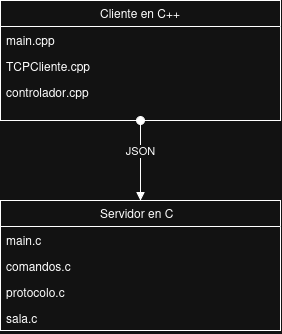
\includegraphics[width=0.34\textwidth]{EstructuraGeneral.drawio.png}
    \label{fig:arquitectura}
\end{figure}
Esto representa como funciona cada parte a grandes rasgos, ya que en 
arquitectura esta un diagrama más específico de todo lo que hace el 
proyecto.
\subsection{Diagrama de clases}
\begin{figure}[H]
    \centering
    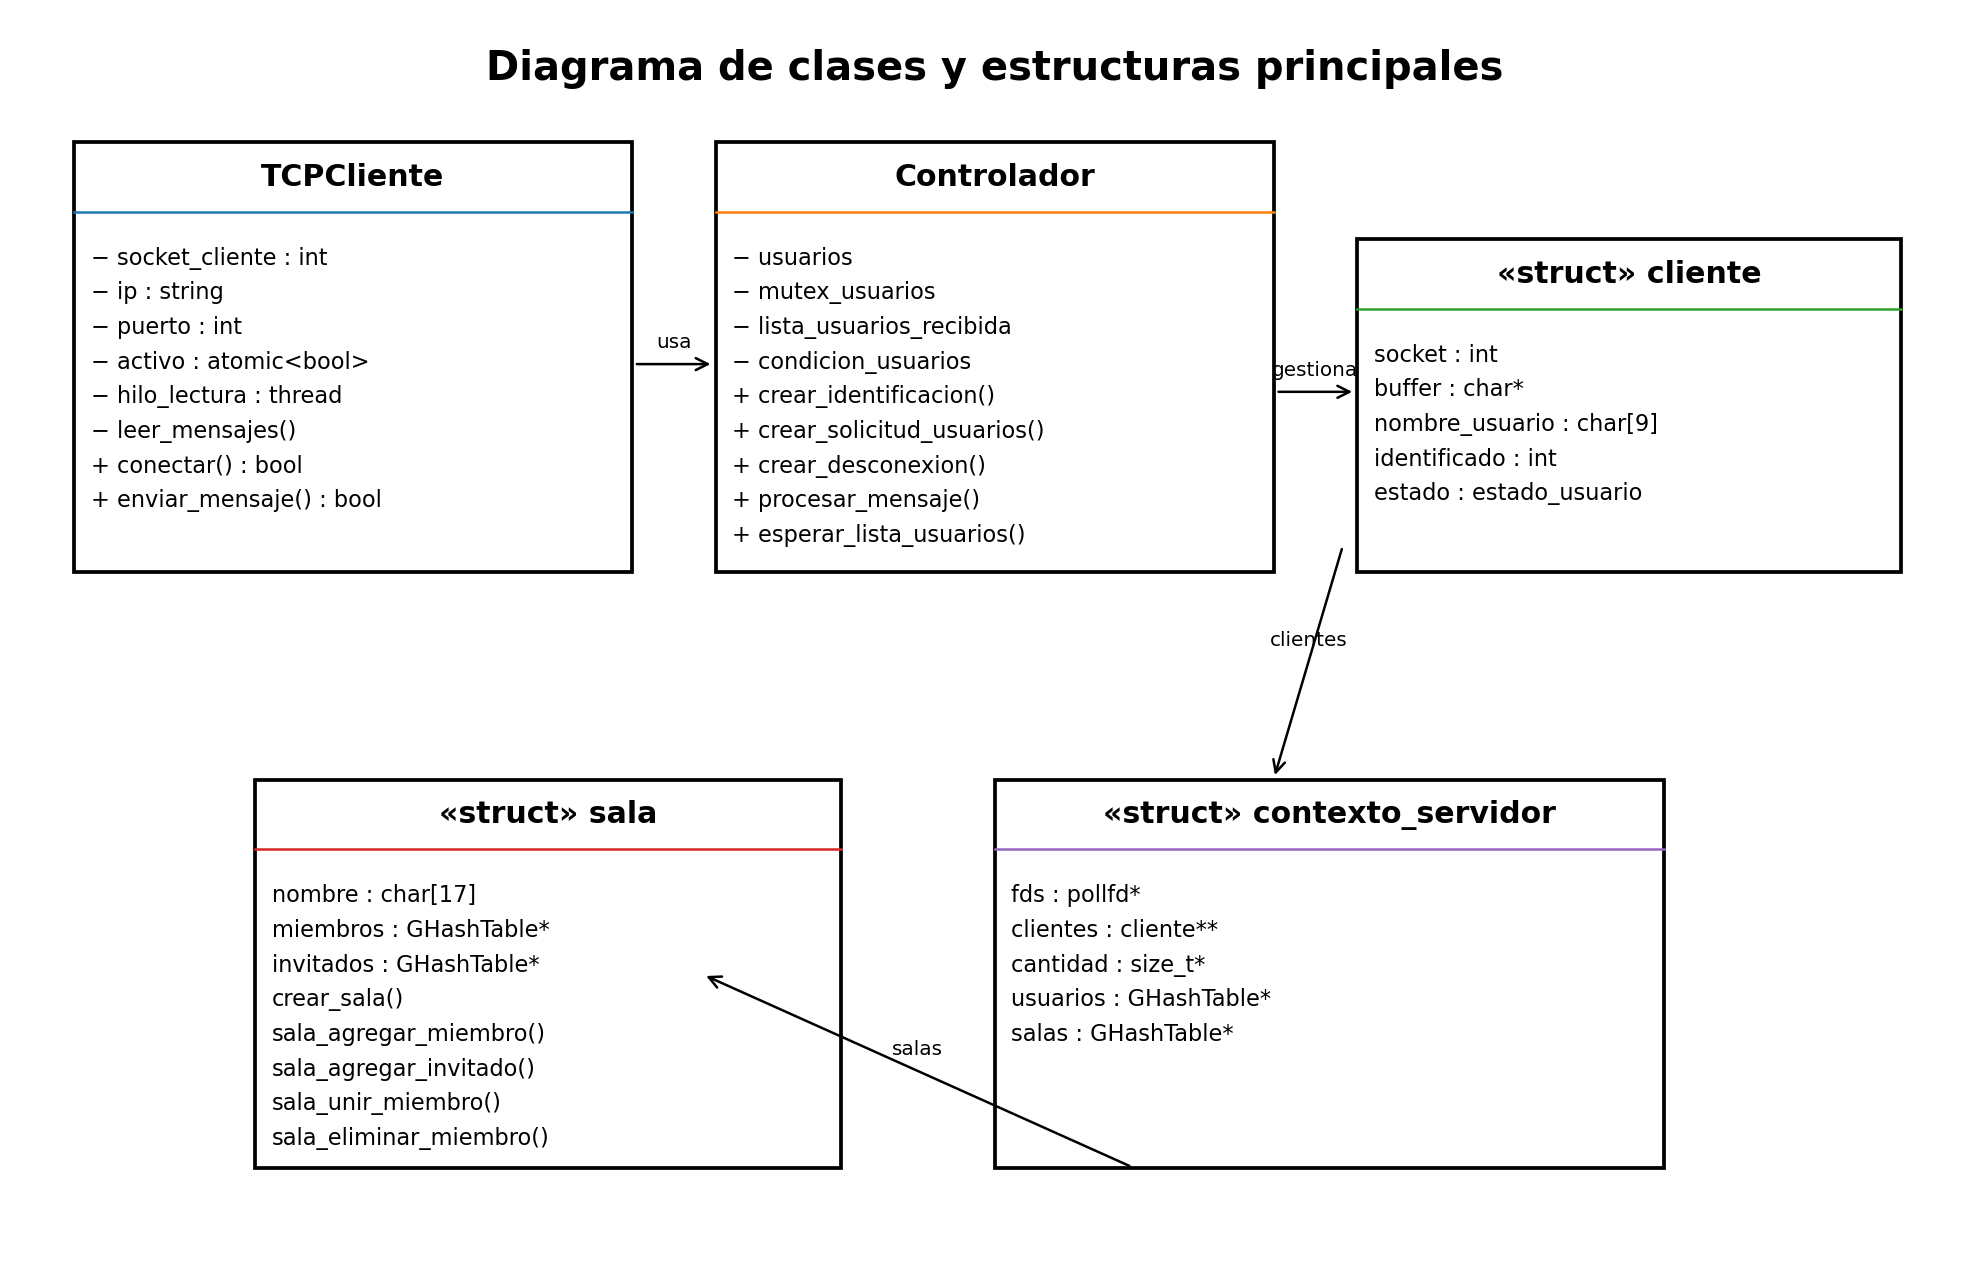
\includegraphics[width=0.75\textwidth]{diagrama_clases_chat.png}
    \label{fig:arquitectura}
\end{figure}
Este diagrama muestra las principales clases y estructuras utilizadas en el proyecto, 
junto con sus responsabilidades y relaciones. Permite observar cómo se organiza internamente 
el cliente y el servidor y qué función cumple cada elemento dentro del sistema.

\subsection{Diagrama de secuencia}
\begin{figure}[H]
    \centering
    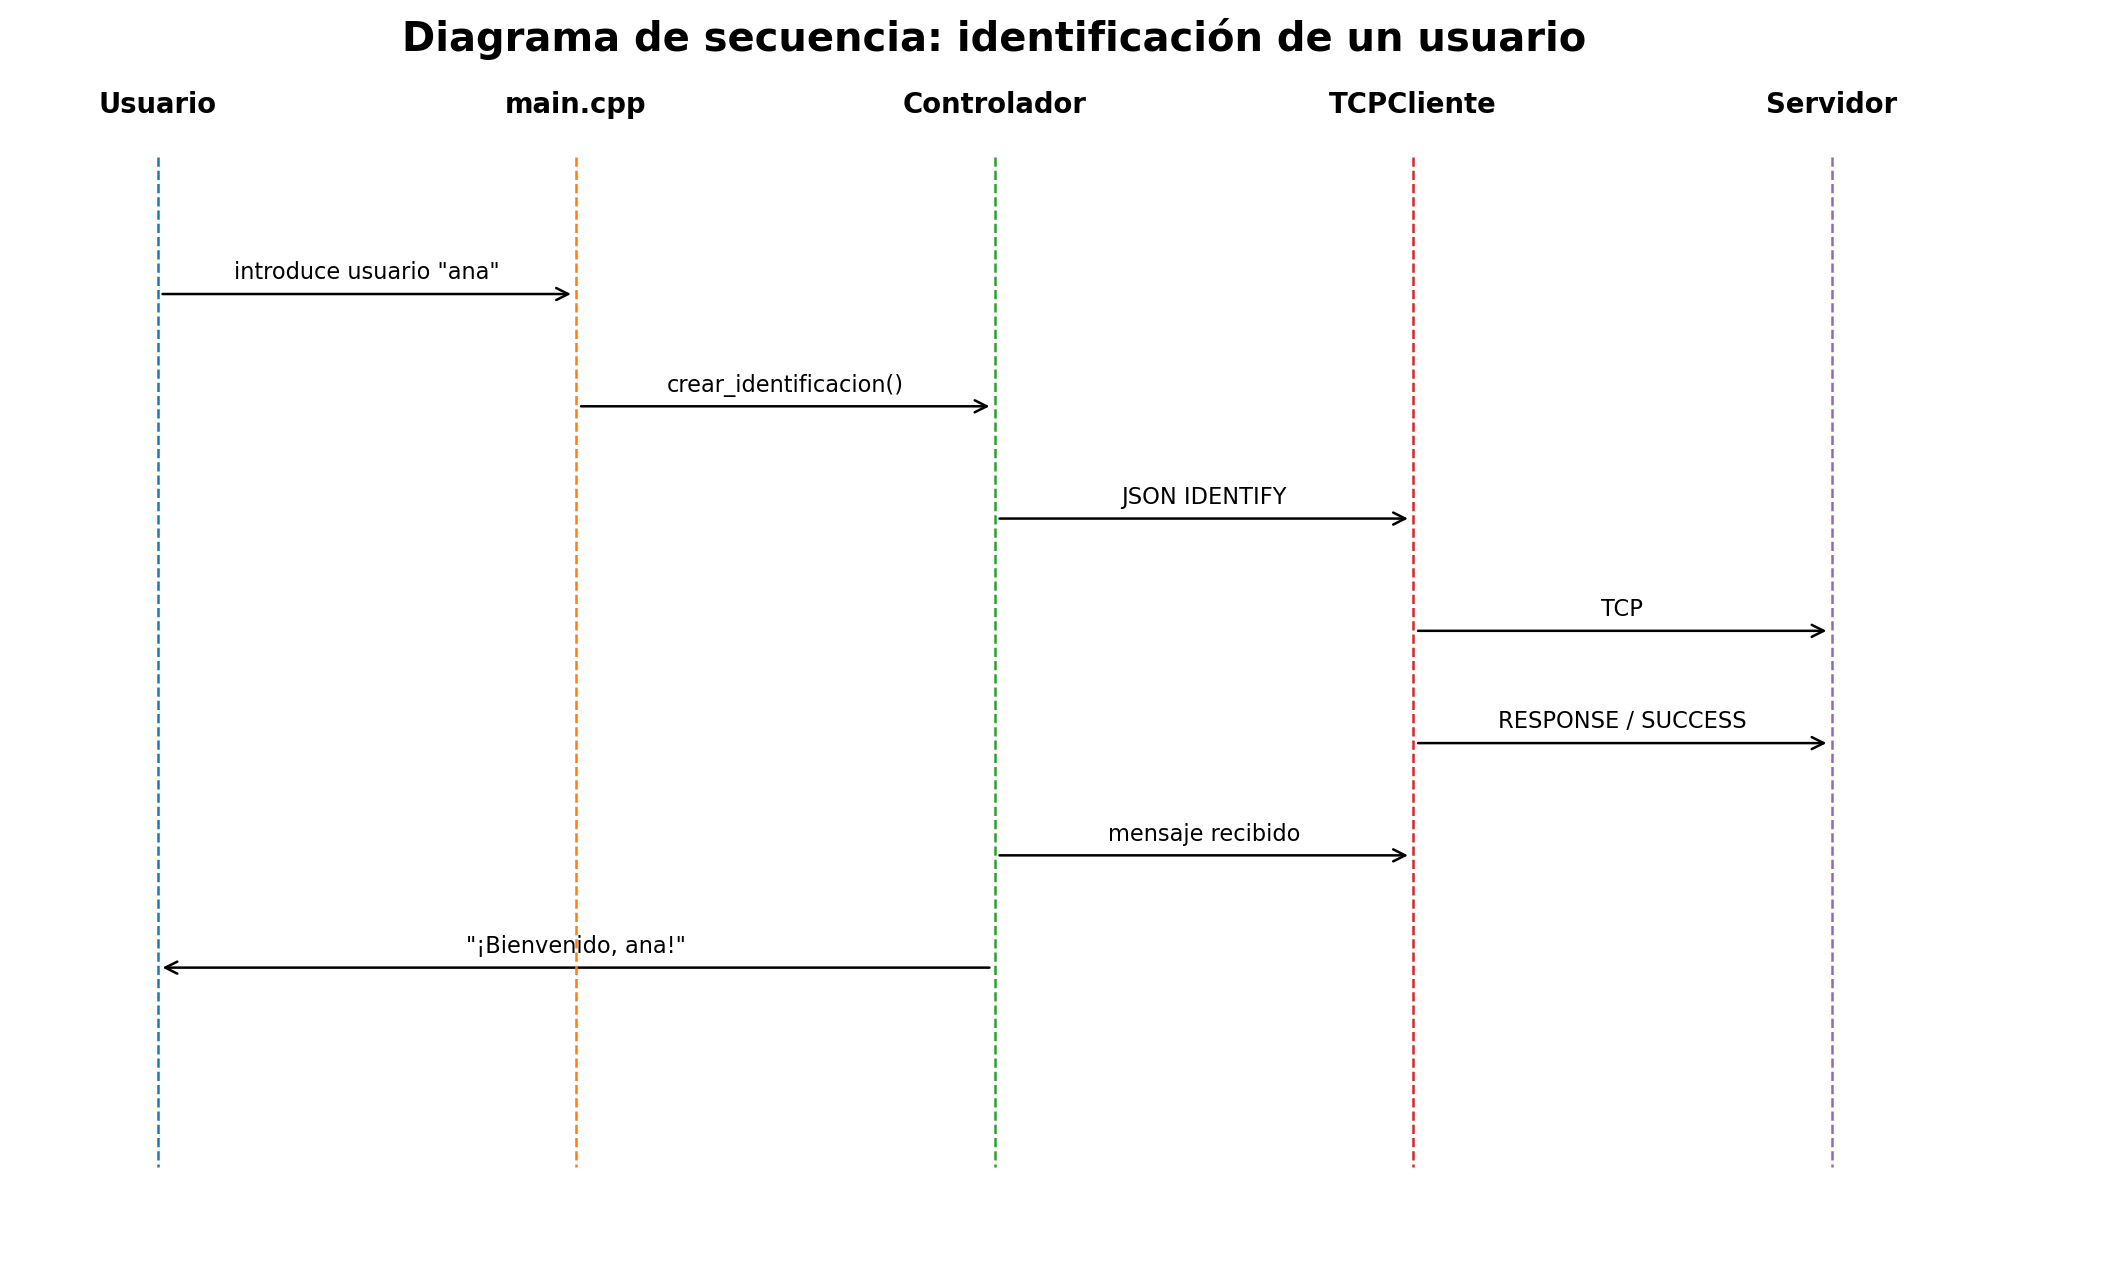
\includegraphics[width=0.75\textwidth]{diagrama_secuencia_identify.png}
    \label{fig:arquitectura}
\end{figure}
Este diagrama muestra la secuencia de comunicación entre el cliente y el servidor durante una 
operación del sistema. Se pueden observar los mensajes que se intercambian, el procesamiento realizado
 por el servidor y la respuesta que recibe el cliente. También permite representar el funcionamiento del 
 hilo encargado de recibir los mensajes en el cliente.

\section{Problemas encontrados y soluciones}

\subsection{Problema 1}
El primer gran problema fue que no sabía utilizar GitHub y cada vez 
que hacía commits me pedía mi usuario y contraseña.

\subsubsection{Solución}
Afortunadamente Miriam mandó al telegram un tutorial para solucionar esto 
y me permitió hacer commits de una forma más eficiente.

\subsection{Problema 2}
Escoger el lenguaje de programación C.\\
En algún punto sentía que por más código que escribía no estaba haciendo
realmente nada y me sentía bastante frustrado porque era culpa del 
lenguaje de programación que escogí.

\subsubsection{Solución}
No hay solución, desde hoy soy hater \#1 de C y no pienso volver a 
utilizarlo nunca más.

\subsection{Problema 3}
No sabía exactamente como comenzar y los tutoriales eran poco claros,
además la parte del servidor era la que más dudas me generaba.

\subsubsection{Solución}
Tuve que buscar más referencias y empezar a combinar todas las cosas
que veía que podían ser útiles para mi proyecto, ya que no todo el 
código que utilizaba de referencia por parte de los repositorios me era
útil.

\subsection{Problema 4}
Me costó bastante la parte de JSON.
Era algo completamente nuevo y hubo muchas veces que no salían los mensajes
como lo planeaba, esto no se llegó a reflejar tanto porque solo hacía commit
cuando compilaba, pero creo que todo lo relacionado a JSON fue bastante 
complicado al comienzo.

\subsubsection{Solución}
Prueba y error, además de tomar bastante de guía los ejemplos que venían
en el protocolo.

\subsection{Problema 5}
Saturar mi main. 
Creo que fue el problema más grande que llegué a tener, conforme iba
avanzando veía que el main crecía más y aunque traté de separarlo no
llegaba a encontrar el momento adecuado y sentía que si lo movía se iba
a romper todo, así que prioricé terminar para después refactorizar.
\subsubsection{Solución}
Leí la página que compartió Miriam y utilicé la más conveniente en mi
caso para así dejar el main más limpio.

\subsection{Problema 6}
Creaba copias de las listas de usuarios en lugar de utilizar la original
con ayuda de los apuntadores.

\subsubsection{Solución}
Esta fue complicado pero no tanto, ya que Canek mencinó en la clase
como debíamos abordar este problema y justamente acababa de implementarlo,
entonces no me fue difícil cambiar todo antes de que fuera demasiado tarde.

\section{Conclusiones}
Al momento de comenzar creí que tendría tiempo suficiente para terminarlo, 
sin embargo, me dí cuenta que era bastante más pesado de completar de lo
que había imaginado. En un inicio tenía pensado hacer interfaz gráfica y
hacer tests, pero conforme avanzaba me quede sin tiempo y tuve que
desvelarme para terminar a tiempo con la fecha de entrega del viernes.\\
Al final fue un proyecto en el que tuve que investigar muchas cosas y
algunas otras copiarlas porque no sabía exactamente como implementarlas,
sin embargo, hubo un punto en el que era más copiar y pegar de las cosas
que ya tenía y eso facilito bastante a la hora de terminar con todo lo que 
pedía el protocolo.\\ 
Aprendí que a C no se le tiene miedo, se le tiene respeto.

\section{Referencias}

\begin{itemize}
    \item Deitel, H. M., \& Deitel, P. J. (2004). \textit{Cómo programar en C, C++ y Java}. Prentice Hall.
    \item Beej's Guide to Network Programming: \url{https://beej.us/guide/bgnet0/}
    \item Building a Simple TCP Chat Application in C:\\ \url{https://medium.com/@trish07/building-a-simple-tcp-chat-application-in-c-a-step-by-step-tutorial-ed3845607d16}
    \item Understanding TCP and Building our Own TCP Server in C:\\ \url{https://medium.com/@shivambhadani_/understanding-tcp-and-building-our-own-tcp-server-in-c-language-8de9d9de78ef}
    \item IBM Documentation, \textit{Using poll() instead of select()}:\\ \url{https://www.ibm.com/docs/en/i/7.4.0?topic=designs-using-poll-instead-select}
    \item AmineToualbi, \textit{TCPChat} (repositorio de referencia):\\ \url{https://github.com/AmineToualbi/TCPChat.git}
    \item BaseMax, \textit{TCP-Chat-CPP} (repositorio de referencia): \\\url{https://github.com/BaseMax/TCP-Chat-CPP.git}
    \item JimmyWorks, \textit{TCP-Chat-App} (repositorio de referencia):\\ \url{https://github.com/JimmyWorks/TCP-Chat-App.git}
    \item JSON, \textit{JSON.org}: \url{https://www.json.org/json-es.html}
    \item Documentación oficial de json-c:\\ \url{https://github.com/json-c/json-c} (API: \url{https://json-c.github.io/json-c/})
    \item Documentación oficial de GLib:\\ \url{https://docs.gtk.org/glib/}
\end{itemize}

\appendix

\end{document}